\documentclass[tikz,border=4pt]{standalone}
\usepackage{pgfplots}
\usepgfplotslibrary{groupplots}
\pgfplotsset{compat=1.18}
\definecolor{proposedblue}{RGB}{46,94,170}
\definecolor{staticgray}{RGB}{128,136,148}
\definecolor{oraclegreen}{RGB}{69,145,98}
\definecolor{blackboxorange}{RGB}{218,132,55}
\definecolor{nomarginred}{RGB}{186,78,68}
\definecolor{vacationgold}{RGB}{204,151,55}
\definecolor{monepurple}{RGB}{126,93,159}
\definecolor{tealgreen}{RGB}{35,143,135}
\definecolor{deepviolet}{RGB}{98,80,154}
\begin{document}

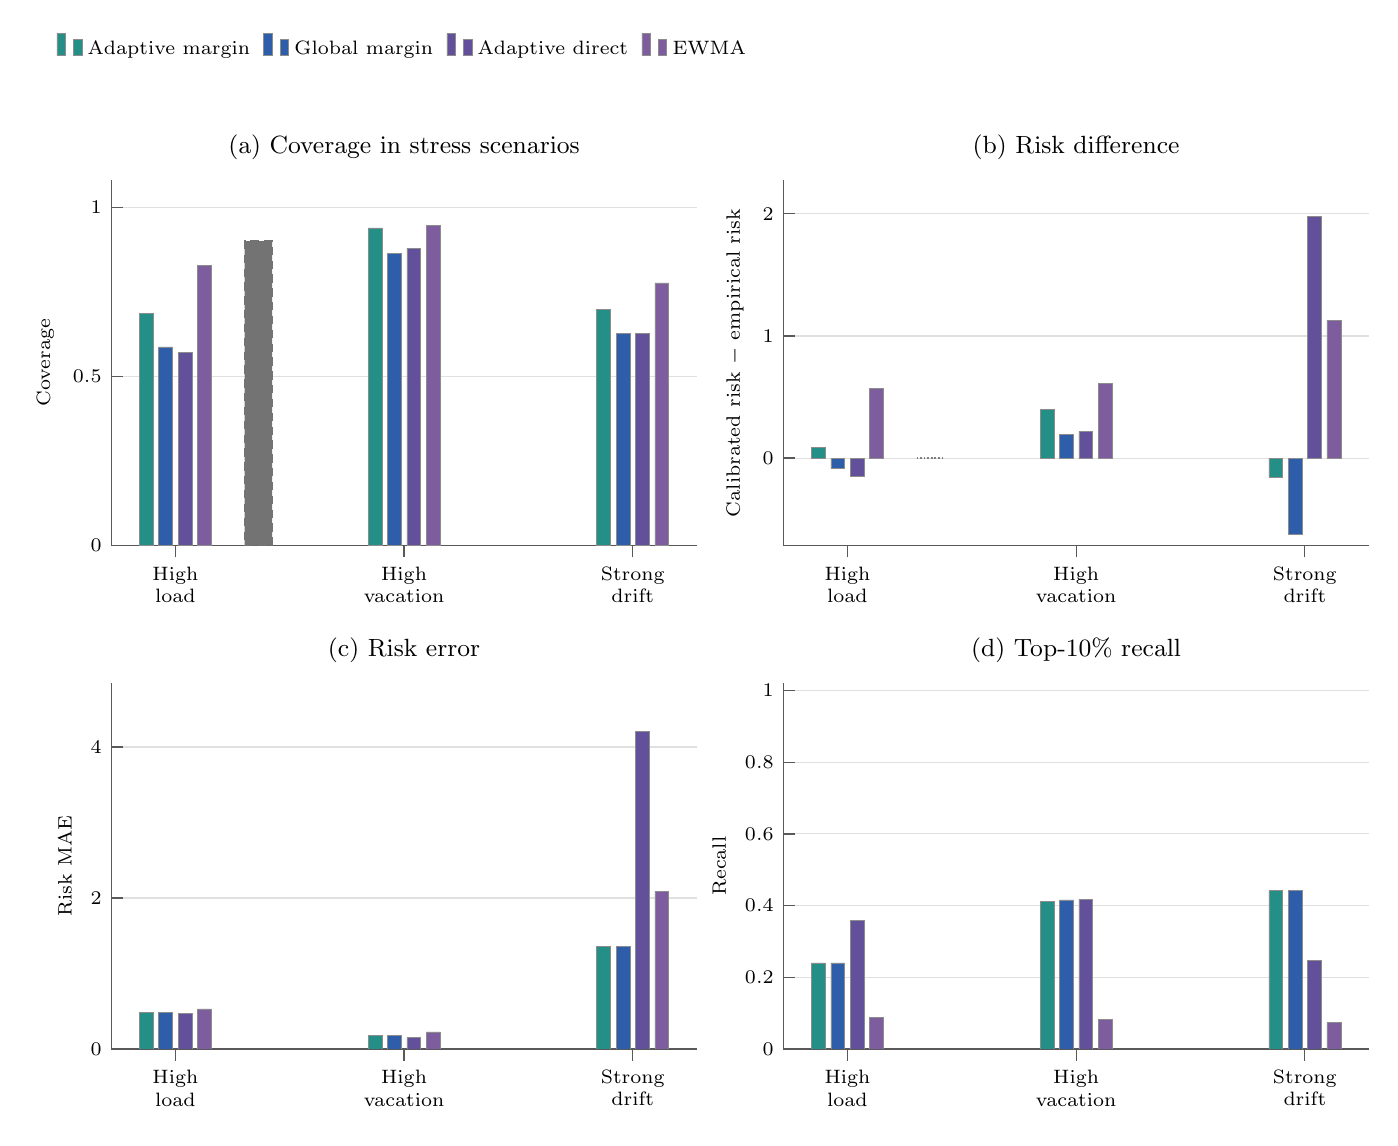
\begin{tikzpicture}
\begin{groupplot}[
    group style={group size=2 by 2, horizontal sep=1.10cm, vertical sep=1.75cm},
    width=3.55in,
    height=2.45in,
    ymajorgrids=true,
    grid style={black!12},
    axis x line*=bottom,
    axis y line*=left,
    axis line style={black!65, line width=0.45pt},
    tick style={black!65, line width=0.45pt},
    label style={font=\scriptsize},
    tick label style={font=\scriptsize},
    title style={font=\small, yshift=-0.5ex},
]
\nextgroupplot[
    title={(a) Coverage in stress scenarios},
    ybar,
    ymin=0.000,
    ymax=1.080,
    ylabel={Coverage},
    legend style={at={(0.5,1.30)}, anchor=south, legend columns=4, draw=none, fill=none, font=\scriptsize, /tikz/every even column/.append style={column sep=0.10cm}},
    symbolic x coords={load_high,vacation_high,drift_strong},
    xtick=data,
    xticklabels={{High\\load},{High\\vacation},{Strong\\drift}},
    x tick label style={font=\scriptsize, align=center, text depth=0.25ex},
    enlarge x limits=0.14,
]
\addplot+[
    ybar,
    bar width=5.0pt,
    fill=tealgreen,
    draw=black!45,
    line width=0.2pt
] coordinates {
(load_high,0.6854)
(vacation_high,0.9388)
(drift_strong,0.6986)
};
\addlegendentry{Adaptive margin}

\addplot+[
    ybar,
    bar width=5.0pt,
    fill=proposedblue,
    draw=black!45,
    line width=0.2pt
] coordinates {
(load_high,0.5870)
(vacation_high,0.8640)
(drift_strong,0.6278)
};
\addlegendentry{Global margin}

\addplot+[
    ybar,
    bar width=5.0pt,
    fill=deepviolet,
    draw=black!45,
    line width=0.2pt
] coordinates {
(load_high,0.5708)
(vacation_high,0.8794)
(drift_strong,0.6266)
};
\addlegendentry{Adaptive direct}

\addplot+[
    ybar,
    bar width=5.0pt,
    fill=monepurple,
    draw=black!45,
    line width=0.2pt
] coordinates {
(load_high,0.8272)
(vacation_high,0.9470)
(drift_strong,0.7766)
};
\addlegendentry{EWMA}

\addplot+[black!55, densely dashed, line width=0.6pt, mark=none, forget plot] coordinates {(load_high,0.9000) (drift_strong,0.9000)};

\nextgroupplot[
    title={(b) Risk difference},
    ybar,
    ymin=-0.717,
    ymax=2.276,
    ylabel={Calibrated risk $-$ empirical risk},
    symbolic x coords={load_high,vacation_high,drift_strong},
    xtick=data,
    xticklabels={{High\\load},{High\\vacation},{Strong\\drift}},
    x tick label style={font=\scriptsize, align=center, text depth=0.25ex},
    enlarge x limits=0.14,
]
\addplot+[
    ybar,
    bar width=5.0pt,
    fill=tealgreen,
    draw=black!45,
    line width=0.2pt
] coordinates {
(load_high,0.0905)
(vacation_high,0.3978)
(drift_strong,-0.1563)
};


\addplot+[
    ybar,
    bar width=5.0pt,
    fill=proposedblue,
    draw=black!45,
    line width=0.2pt
] coordinates {
(load_high,-0.0857)
(vacation_high,0.1910)
(drift_strong,-0.6236)
};


\addplot+[
    ybar,
    bar width=5.0pt,
    fill=deepviolet,
    draw=black!45,
    line width=0.2pt
] coordinates {
(load_high,-0.1500)
(vacation_high,0.2188)
(drift_strong,1.9790)
};


\addplot+[
    ybar,
    bar width=5.0pt,
    fill=monepurple,
    draw=black!45,
    line width=0.2pt
] coordinates {
(load_high,0.5710)
(vacation_high,0.6108)
(drift_strong,1.1268)
};


\addplot+[black!50, dotted, line width=0.6pt, mark=none, forget plot] coordinates {(load_high,0) (drift_strong,0)};

\nextgroupplot[
    title={(c) Risk error},
    ybar,
    ymin=0.000,
    ymax=4.843,
    ylabel={Risk MAE},
    symbolic x coords={load_high,vacation_high,drift_strong},
    xtick=data,
    xticklabels={{High\\load},{High\\vacation},{Strong\\drift}},
    x tick label style={font=\scriptsize, align=center, text depth=0.25ex},
    enlarge x limits=0.14,
]
\addplot+[
    ybar,
    bar width=5.0pt,
    fill=tealgreen,
    draw=black!45,
    line width=0.2pt
] coordinates {
(load_high,0.4853)
(vacation_high,0.1752)
(drift_strong,1.3619)
};


\addplot+[
    ybar,
    bar width=5.0pt,
    fill=proposedblue,
    draw=black!45,
    line width=0.2pt
] coordinates {
(load_high,0.4853)
(vacation_high,0.1752)
(drift_strong,1.3619)
};


\addplot+[
    ybar,
    bar width=5.0pt,
    fill=deepviolet,
    draw=black!45,
    line width=0.2pt
] coordinates {
(load_high,0.4724)
(vacation_high,0.1496)
(drift_strong,4.2114)
};


\addplot+[
    ybar,
    bar width=5.0pt,
    fill=monepurple,
    draw=black!45,
    line width=0.2pt
] coordinates {
(load_high,0.5294)
(vacation_high,0.2250)
(drift_strong,2.0908)
};



\nextgroupplot[
    title={(d) Top-10\% recall},
    ybar,
    ymin=0.000,
    ymax=1.020,
    ylabel={Recall},
    symbolic x coords={load_high,vacation_high,drift_strong},
    xtick=data,
    xticklabels={{High\\load},{High\\vacation},{Strong\\drift}},
    x tick label style={font=\scriptsize, align=center, text depth=0.25ex},
    enlarge x limits=0.14,
]
\addplot+[
    ybar,
    bar width=5.0pt,
    fill=tealgreen,
    draw=black!45,
    line width=0.2pt
] coordinates {
(load_high,0.2400)
(vacation_high,0.4120)
(drift_strong,0.4420)
};


\addplot+[
    ybar,
    bar width=5.0pt,
    fill=proposedblue,
    draw=black!45,
    line width=0.2pt
] coordinates {
(load_high,0.2400)
(vacation_high,0.4160)
(drift_strong,0.4420)
};


\addplot+[
    ybar,
    bar width=5.0pt,
    fill=deepviolet,
    draw=black!45,
    line width=0.2pt
] coordinates {
(load_high,0.3580)
(vacation_high,0.4180)
(drift_strong,0.2480)
};


\addplot+[
    ybar,
    bar width=5.0pt,
    fill=monepurple,
    draw=black!45,
    line width=0.2pt
] coordinates {
(load_high,0.0880)
(vacation_high,0.0820)
(drift_strong,0.0740)
};


\end{groupplot}
\end{tikzpicture}
\end{document}
